\documentclass[11pt,a4paper]{article}

% Packages
\usepackage[utf8]{inputenc}
\usepackage[T1]{fontenc}
\usepackage{mathpazo}  % Palatino for elegant serif
\usepackage{helvet}    % Helvetica for sans in headers
\usepackage{microtype}
\usepackage[hmargin=1.25in,vmargin=1in]{geometry}
\usepackage{amsmath,amssymb}
\usepackage{graphicx}
\usepackage{xcolor}
\usepackage{booktabs}
\usepackage{longtable}
\usepackage{array}
\usepackage{hyperref}
\usepackage{titlesec}
\usepackage{tcolorbox}
\usepackage{listings}
\usepackage{fancyhdr}
\usepackage{enumitem}
\usepackage{tikz}
\usetikzlibrary{shapes.geometric, arrows.meta, positioning, fit}

% Colors
\definecolor{accent}{HTML}{1a5f7a}
\definecolor{accentlight}{HTML}{e8f4f8}
\definecolor{codebg}{HTML}{f6f8fa}
\definecolor{codeborder}{HTML}{e1e4e8}

% Hyperref
\hypersetup{
  colorlinks=true,
  linkcolor=accent,
  urlcolor=accent,
  citecolor=accent,
  pdftitle={Feature Summary — Economics Data Suite},
  pdfauthor={}
}

% Section formatting
\titleformat{\section}
  {\normalfont\sffamily\Large\bfseries\color{accent}}
  {\thesection}{1em}{}[\titlerule]
\titleformat{\subsection}
  {\normalfont\sffamily\large\bfseries}
  {\thesubsection}{1em}{}
\titleformat{\subsubsection}
  {\normalfont\sffamily\normalsize\bfseries}
  {\thesubsubsection}{1em}{}

% Listings for code
\lstdefinestyle{pythonstyle}{
  language=Python,
  basicstyle=\ttfamily\small,
  backgroundcolor=\color{codebg},
  frame=single,
  framerule=0pt,
  rulecolor=\color{codeborder},
  xleftmargin=12pt,
  xrightmargin=12pt,
  framexleftmargin=12pt,
  framexrightmargin=12pt,
  aboveskip=6pt,
  belowskip=6pt,
  keywordstyle=\color{accent}\bfseries,
  commentstyle=\color{gray}\itshape,
  stringstyle=\color{olive},
  showstringspaces=false,
  breaklines=true,
  columns=flexible,
  keepspaces=true,
  escapeinside={(*@}{@*)},
}
\lstset{style=pythonstyle}

% Intuition box
\newtcolorbox{intuitionbox}{
  colback=accentlight,
  colframe=accent,
  fonttitle=\bfseries\sffamily,
  title=Non-technical intuition,
  arc=2pt,
  boxrule=0.5pt,
}

% Header/footer
\pagestyle{fancy}
\fancyhf{}
\fancyhead[L]{\sffamily\small Feature Summary}
\fancyhead[R]{\sffamily\small Economics Data Suite}
\fancyfoot[C]{\thepage}
\renewcommand{\headrulewidth}{0.4pt}
\renewcommand{\footrulewidth}{0.4pt}

\begin{document}

% Title
\begin{titlepage}
  \centering
  \vspace*{2cm}
  {\sffamily\Huge\bfseries\color{accent} Feature Summary\par}
  \vspace{0.5cm}
  {\LARGE Economics Data Suite\par}
  \vspace{2cm}
  \begin{tcolorbox}[colback=accentlight,colframe=accent,width=0.9\textwidth,arc=4pt]
    \centering
    \small
    A comprehensive technical and intuitive guide to every feature in the repository:\\
    providers, recipes, transforms, models, visualization, and infrastructure.
  \end{tcolorbox}
  \vfill
  {\large \today\par}
\end{titlepage}

\tableofcontents
\newpage

%==============================================================================
\section{Executive Overview}
%==============================================================================

This repository is an ``economics data suite'': a small application that helps you (1) \textbf{pull time-series data}, (2) \textbf{transform it} into more meaningful measures (growth, inflation, spreads, returns), (3) \textbf{run simple econometric models} (OLS, AR(1), local projections), and (4) \textbf{forecast} and \textbf{visualize} the results.

\vspace{0.5em}
\noindent\textbf{Local-first} means everything runs on your computer (no server you have to deploy). The user interface is built in \textbf{Streamlit}, which is a Python tool for making simple interactive web apps. Under the hood, the project organizes work as \textbf{jobs}: you submit a request (``fetch CPI from FRED'' or ``compute YoY inflation''), the job runs, and the output is saved as a CSV file you can plot or download.

\begin{intuitionbox}
Think of the app as a ``time-series lab notebook.'' You choose a series (like CPI, unemployment, or a stock price), press run, and the app saves a clean dataset plus a record of what you did. You can then build up from raw data to transformed series to models and forecasts.
\end{intuitionbox}

\noindent\textbf{Two main modes:}
\begin{itemize}[leftmargin=2em]
  \item \textbf{Finance}: market tickers (prices/volume), technical indicators, and forecasting tools.
  \item \textbf{Econ}: FRED macro series, macro transforms, and econometric models.
\end{itemize}

\noindent\textbf{Dataset Builder}: a UI that merges multiple series into one aligned dataset (same date column), which is usually the first step before running regressions.

\vspace{0.5em}
\noindent\textbf{What this document is:} a guided explanation of the data flow and the main methods, followed by a per-feature reference (each provider/recipe) with code snippets.

%==============================================================================
\section{Architecture \& Data Flow}
%==============================================================================

\begin{center}
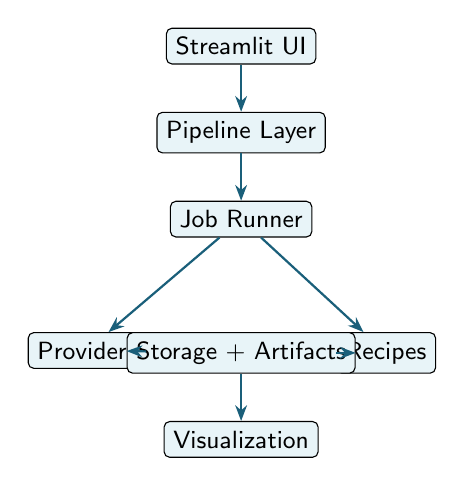
\begin{tikzpicture}[
  node distance=0.6cm and 1.2cm,
  box/.style={rectangle, draw, rounded corners=2pt, fill=accentlight, font=\small\sffamily},
  subbox/.style={rectangle, draw, rounded corners=2pt, fill=white, font=\scriptsize},
  arrow/.style={-{Stealth[length=2mm]}, thick, color=accent}
]
  \node[box] (ui) {Streamlit UI};
  \node[box, below=of ui] (pipe) {Pipeline Layer};
  \node[box, below=of pipe] (jobs) {Job Runner};
  \node[box, below left=1.2cm and 0.3cm of jobs] (prov) {Providers};
  \node[box, below right=1.2cm and 0.3cm of jobs] (rec) {Recipes};
  \node[box, below=1.2cm of jobs] (store) {Storage + Artifacts};
  \node[box, below=of store] (viz) {Visualization};

  \draw[arrow] (ui) -- (pipe);
  \draw[arrow] (pipe) -- (jobs);
  \draw[arrow] (jobs) -- (prov);
  \draw[arrow] (jobs) -- (rec);
  \draw[arrow] (prov) -- (store);
  \draw[arrow] (rec) -- (store);
  \draw[arrow] (store) -- (viz);
\end{tikzpicture}
\end{center}

\textbf{Flow (big picture):} UI submits provider fetches and recipe runs $\to$ JobRunner executes (in background threads) $\to$ Providers fetch raw data and Recipes transform/model it $\to$ SQLite stores job status/logs, and CSV artifacts store results $\to$ Plotly renders charts (optionally with recession shading).

\vspace{0.5em}
\noindent\textbf{Step-by-step: what happens when you click ``Run'':}
\begin{enumerate}[leftmargin=2.2em]
  \item \textbf{You choose an input}: a ticker (Finance) or a FRED series ID (Econ), plus dates and options.
  \item \textbf{The app creates a job}: a new row in the SQLite database with status \texttt{QUEUED}.
  \item \textbf{A worker executes the job}: the JobRunner calls either a provider (to fetch data) or a recipe (to transform/model an existing dataset).
  \item \textbf{Results are saved}: if the job succeeds, its output DataFrame is written to a CSV file (an ``artifact'') in the results directory.
  \item \textbf{You inspect and plot}: the UI reads the artifact, renders charts, and lets you download the CSV.
\end{enumerate}

\begin{intuitionbox}
The job system is there so the UI stays responsive. Instead of doing everything immediately in the button click, the app records ``what to do'' and runs it in the background, then updates the results when finished.
\end{intuitionbox}

%==============================================================================
\section{Configuration \& Feature Gating}
%==============================================================================

\begin{tabular}{@{}ll@{}}
  \toprule
  \textbf{Env Var} & \textbf{Purpose} \\
  \midrule
  \texttt{FINREC\_DB\_PATH} & SQLite database path (default: \texttt{data/finrec.db}) \\
  \texttt{FINREC\_RESULTS\_DIR} & CSV artifact output directory (default: \texttt{data/results}) \\
  \texttt{FINREC\_FMP\_API\_KEY} & API key for FMP provider (required when using \texttt{fmp}) \\
  \bottomrule
\end{tabular}

\vspace{0.5em}
\textbf{Optional extras} (pyproject.toml): \texttt{dev}, \texttt{market}, \texttt{macro}, \texttt{news}, \texttt{ml}, \texttt{econ}, \texttt{forecast}. Providers and recipes that depend on optional packages are registered only when those packages are installed; runtime calls use \texttt{require\_optional()} and raise a friendly install hint if missing.

%==============================================================================
\section{Getting Started (Runbook)}
%==============================================================================

\textbf{Goal:} get the Streamlit UI running locally, then run a first end-to-end workflow.

\subsection{Install and run}
\begin{enumerate}[leftmargin=2.2em]
  \item Create and activate a Python environment.
  \item Install the package (and optional extras if you want specific features).
  \item Create a \texttt{.env} file (copy from \texttt{.env.example}) if you want to change default paths or add an API key.
  \item Start Streamlit: \texttt{streamlit run streamlit\_app.py}.
\end{enumerate}

\subsection{What ``optional extras'' mean}
Some features require heavier libraries (for example \texttt{statsmodels} for econometrics or \texttt{transformers} for FinBERT sentiment). To keep installation light, those are optional. If you try to use a feature without its dependency installed, the app will raise a message telling you which extra to install, e.g.:
\[
\texttt{pip install -e ".[forecast]"}
\]

\subsection{Where outputs live}
\begin{itemize}[leftmargin=2em]
  \item \textbf{SQLite database}: stores job metadata, status, and logs (default: \texttt{data/finrec.db}).
  \item \textbf{CSV artifacts}: each successful job writes \texttt{\{job\_id\}.csv} to the results directory (default: \texttt{data/results/}).
\end{itemize}

%==============================================================================
\section{Core Concepts (the minimal vocabulary)}
%==============================================================================

\begin{description}[leftmargin=2.5em, style=nextline]
  \item[Time series] A dataset where each observation has a date/time (monthly CPI, daily stock prices, quarterly GDP).
  \item[Provider] A data source connector that \textit{fetches raw data} (market prices, FRED macro series, news articles).
  \item[Recipe] A transformation or model that \textit{takes a dataset} and produces a new dataset (inflation, returns, OLS results, forecasts).
  \item[Job] A run of a provider or recipe, tracked with an ID, status, logs, and (if it succeeds) an output CSV artifact.
  \item[Artifact] The saved output CSV from a job. Artifacts are the main ``inputs'' to later steps.
\end{description}

\begin{intuitionbox}
If you remember one idea: providers \(\rightarrow\) recipes \(\rightarrow\) artifacts. You start with raw series, compute transformed series, and then run models/forecasts on those transformed series.
\end{intuitionbox}

%==============================================================================
\section{High-Level Methods Overview (why these features exist)}
%==============================================================================

\subsection{Macro transforms (inflation, growth, spreads, real rates)}
Economists often transform raw levels into rates of change or differences. For example:
\begin{itemize}[leftmargin=2em]
  \item \textbf{Inflation} is the growth rate of a price index (CPI). Year-over-year rates help smooth seasonal noise.
  \item \textbf{Growth rates} of output (GDP) are often annualized to make numbers comparable across frequencies.
  \item \textbf{Spreads} (like 10-year minus 2-year yields) summarize information about the yield curve.
  \item \textbf{Real rates} subtract inflation from nominal rates to approximate inflation-adjusted returns.
\end{itemize}
These transforms are implemented as recipes so you can compute them consistently and save the result as a new artifact.

\subsection{Econometrics (OLS, AR(1), local projections/IRFs)}
This app includes a small set of ``workhorse'' models:
\begin{itemize}[leftmargin=2em]
  \item \textbf{OLS} estimates a linear relationship between a dependent variable and one or more predictors.
  \item \textbf{AR(1)} is the simplest persistence model for a single series: today depends on yesterday.
  \item \textbf{Local projections (IRFs)} estimate how a variable responds over time to a shock.
\end{itemize}
\textit{Important:} these tools help you explore and learn, but they do not automatically solve identification or causal inference. Interpretation should be cautious.

\subsection{Forecasting (baselines, statistical models, and ML lags)}
Forecasting is useful when you want a simple quantitative guess about future values, or when you want to compare methods. The suite includes:
\begin{itemize}[leftmargin=2em]
  \item \textbf{Baselines} (naive, drift): fast, easy benchmarks.
  \item \textbf{Statistical models} (ETS, ARIMA): common time-series forecasting methods with uncertainty intervals.
  \item \textbf{Lag-based ML} (ridge, random forest): supervised learning on lagged values; can capture nonlinear patterns but can also overfit.
\end{itemize}

\subsection{Technical indicators and news sentiment}
\begin{itemize}[leftmargin=2em]
  \item \textbf{Technical indicators} (SMA/EMA/RSI/MACD/volatility) summarize price momentum, trend, and variability. They are descriptive features, not ``proof'' of predictability.
  \item \textbf{News sentiment} converts article text into a numeric score (positive/negative) and aggregates it by day, so you can treat it like another time series.
\end{itemize}

%==============================================================================
\section{Worked Examples (end-to-end workflows)}
%==============================================================================

\subsection{Example A: CPI to YoY inflation to plot}
\textbf{Question:} ``How has inflation evolved over time?'' A common starting point is CPI inflation year-over-year.
\begin{enumerate}[leftmargin=2.2em]
  \item In \textbf{Econ} mode, fetch CPI from FRED (e.g., \texttt{CPIAUCSL}) over a long date range.
  \item Run the \textbf{InflationYoYRecipe} on the fetched CPI artifact.
  \item Plot the resulting YoY series and compare peaks/troughs across time.
\end{enumerate}
\begin{intuitionbox}
YoY inflation answers: ``Compared to the same month last year, how much higher is the price level today?'' This helps avoid misleading month-to-month noise.
\end{intuitionbox}

\subsection{Example B: a series to baseline forecasts to ARIMA}
\textbf{Question:} ``If I had to project this series forward, what would simple methods say?''\newline
Workflow:
\begin{enumerate}[leftmargin=2.2em]
  \item Choose a target series (macro series or a price series).
  \item Run \textbf{Naive} and \textbf{Drift} forecasts first. These are baselines: if a fancy model cannot beat them, that is a warning sign.
  \item Run \textbf{ARIMA}. Look at the forecast path and (if provided) the confidence interval to understand uncertainty.
\end{enumerate}
\begin{intuitionbox}
Forecast evaluation is hard. This app’s goal is to make it easy to compare methods in a consistent pipeline, not to claim any one method is ``best'' in general.
\end{intuitionbox}

\subsection{Example C: build a regression dataset, run OLS, interpret}
\textbf{Question:} ``How does inflation relate to interest rates (in this sample)?''\newline
This example emphasizes workflow and interpretation rather than causal claims.
\begin{enumerate}[leftmargin=2.2em]
  \item Fetch two series from FRED (for example, CPI to build inflation and a nominal rate series).
  \item Use recipes to transform them into comparable units (e.g., inflation YoY and a nominal rate in percent).
  \item Use the \textbf{Dataset Builder} to merge the two artifacts into one dataset with aligned dates.
  \item Run \textbf{OLSRecipe} with inflation as \(y\) and the nominal rate as \(x\) (or vice versa).
  \item Interpret the coefficient as an \textbf{association} within the sample and check the standard error and p-value for uncertainty.
\end{enumerate}
\begin{intuitionbox}
OLS can tell you ``when \(x\) is higher, does \(y\) tend to be higher too?'' But it does not automatically tell you why. For causal interpretation, you need a research design (identification) beyond a simple regression.
\end{intuitionbox}

%==============================================================================
\section{Glossary (quick definitions)}
%==============================================================================

\begin{description}[leftmargin=2.8em, style=nextline]
  \item[OHLCV] Open, High, Low, Close, Volume. A common daily stock-price dataset format.
  \item[Return] A change in value from one period to the next. In finance, returns are often modeled instead of prices.
  \item[Log return] \(\ln(p_t) - \ln(p_{t-1})\). Approximately the percent change (in decimals) for small changes.
  \item[Annualized] Scaled to ``per year'' units. Example: monthly log change \(\times 12 \times 100\) becomes annualized percent.
  \item[Lag] A past value of a series, like \(y_{t-1}\).
  \item[Horizon] How far ahead you forecast or measure a response (e.g., 6 months ahead).
  \item[Train/test split] A common forecasting workflow: fit the model on earlier data (train) and evaluate on later data (test).
  \item[Stationary] Roughly: a series whose statistical properties (mean/variance) do not change over time. Many models behave better on stationary series.
  \item[AIC] Akaike Information Criterion. A metric that trades off fit vs model complexity; lower is better in-sample under the criterion.
  \item[Standard error] An estimate of the uncertainty (sampling variability) of a coefficient estimate.
  \item[p-value] Under the model assumptions, the probability of seeing a \(t\)-statistic as extreme as observed if the true coefficient were 0.
  \item[Confidence interval] A range of plausible values for a parameter or forecast, under model assumptions.
  \item[IRF] Impulse Response Function: the response of a variable over time after a one-time shock.
\end{description}

%==============================================================================
\section{Reference: Feature Index}
%==============================================================================

\begin{longtable}{@{}cllc@{}}
  \toprule
  \# & \textbf{Feature} & \textbf{Category} & \textbf{Ref} \\
  \midrule
  \endfirsthead

  \multicolumn{4}{l}{\textit{Continued from previous page}} \\
  \toprule
  \# & \textbf{Feature} & \textbf{Category} & \textbf{Ref} \\
  \midrule
  \endhead

  \bottomrule
  \multicolumn{4}{r}{\textit{Continued on next page}} \\
  \endfoot

  \bottomrule
  \endlastfoot

  1 & YFinanceProvider & Data Ingestion & \ref{sec:yfinance} \\
  2 & FMPProvider & Data Ingestion & \ref{sec:fmp} \\
  3 & FREDProvider & Data Ingestion & \ref{sec:fred} \\
  4 & GDELTProvider & Data Ingestion & \ref{sec:gdelt} \\
  5 & ProviderRegistry & Infra & \ref{sec:provider-registry} \\
  6 & Provider base protocol & Infra & \ref{sec:provider-base} \\
  7 & NaiveForecastRecipe & Forecasting & \ref{sec:naive} \\
  8 & DriftForecastRecipe & Forecasting & \ref{sec:drift} \\
  9 & ETSForecastRecipe & Forecasting & \ref{sec:ets} \\
  10 & ARIMAForecastRecipe & Forecasting & \ref{sec:arima} \\
  11 & RidgeLagForecastRecipe & Forecasting & \ref{sec:ridge} \\
  12 & RandomForestLagForecastRecipe & Forecasting & \ref{sec:rf} \\
  13 & Forecast utilities & Infra & \ref{sec:forecast-utils} \\
  14 & InflationYoYRecipe & Macro Transform & \ref{sec:inflation-yoy} \\
  15 & InflationMoMAnnRecipe & Macro Transform & \ref{sec:inflation-mom} \\
  16 & GrowthQoQAnnRecipe & Macro Transform & \ref{sec:growth-qoq} \\
  17 & SpreadRecipe & Macro Transform & \ref{sec:spread} \\
  18 & RealRateRecipe & Macro Transform & \ref{sec:real-rate} \\
  19 & OLSRecipe & Econometrics & \ref{sec:ols} \\
  20 & AR1Recipe & Econometrics & \ref{sec:ar1} \\
  21 & LocalProjectionIRFRecipe & Econometrics & \ref{sec:lp-irf} \\
  22 & FinBERTDailySentimentRecipe & News & \ref{sec:finbert} \\
  23 & SimpleMovingAverageRecipe & Technical & \ref{sec:sma} \\
  24 & ExponentialMovingAverageRecipe & Technical & \ref{sec:ema} \\
  25 & RSIRecipe & Technical & \ref{sec:rsi} \\
  26 & MACDRecipe & Technical & \ref{sec:macd} \\
  27 & RollingVolatilityRecipe & Technical & \ref{sec:rolling-vol} \\
  28 & LogReturnsRecipe & Time Series & \ref{sec:log-returns} \\
  29 & RollingZScoreRecipe & Time Series & \ref{sec:rolling-zscore} \\
  30 & RecipeRegistry & Infra & \ref{sec:recipe-registry} \\
  31 & Recipe base protocol & Infra & \ref{sec:recipe-base} \\
  32 & SQLiteStorage & Storage & \ref{sec:sqlite} \\
  33 & JobRunner & Orchestration & \ref{sec:job-runner} \\
  34 & Pipeline submission & Orchestration & \ref{sec:pipeline} \\
  35 & build\_merged\_dataset & Datasets & \ref{sec:merge} \\
  36 & plot\_timeseries & Visualization & \ref{sec:plot} \\
  37 & build\_recession\_intervals & Visualization & \ref{sec:recession} \\
  38 & Time series catalog & UI & \ref{sec:catalog} \\
  39 & AppConfig / load\_config & Config & \ref{sec:config} \\
  40 & Optional dependency helpers & Infra & \ref{sec:optional} \\
  41 & Main Streamlit app & UI & \ref{sec:streamlit} \\
  42 & Legacy pages & UI & \ref{sec:legacy} \\
  43 & E2E smoke script & Scripts & \ref{sec:e2e} \\
\end{longtable}

\newpage

%==============================================================================
\section{Feature Writeups}
%==============================================================================

\subsection{Data Ingestion}

\subsubsection{YFinanceProvider}\label{sec:yfinance}

\textbf{What it is:} Fetches market OHLCV data via the yfinance library (Yahoo Finance).

\textbf{Technical:} Uses \texttt{yfinance.Ticker(symbol).history()} with date range or fallback \texttt{n} rows. Rate limiting: global throttle (default 3s) and retry with backoff on \texttt{YFRateLimitError}. Output: \texttt{date}, \texttt{symbol}, \texttt{open}, \texttt{high}, \texttt{low}, \texttt{close}, \texttt{volume}.

\textbf{When to use:}
\begin{itemize}[leftmargin=2em]
  \item When you want a free, quick way to pull daily price history for common tickers.
  \item When you want a fallback source if an API provider rejects a symbol (e.g., paywalled endpoints elsewhere).
\end{itemize}

\textbf{Inputs/outputs (practical):}
\begin{itemize}[leftmargin=2em]
  \item \textbf{Input}: a ticker symbol (e.g., \texttt{AAPL}) and a date range (or a row limit).
  \item \textbf{Output}: one row per trading day with OHLCV (Open, High, Low, Close, Volume).
\end{itemize}

\textbf{Common pitfalls:}
\begin{itemize}[leftmargin=2em]
  \item \textbf{Rate limits} happen. If you request too often, Yahoo can temporarily block you; the provider sleeps and retries.
  \item \textbf{Non-trading days}: there is no data on weekends/holidays, so daily series have gaps.
  \item \textbf{Interpretation}: OHLC are prices; to model/forecast, you often want returns (see \ref{sec:log-returns}) rather than raw levels.
\end{itemize}

\textbf{Where:} \texttt{src/finrec/providers/market/yfinance.py} --- \texttt{YFinanceProvider}

\begin{lstlisting}
@dataclass
class YFinanceProvider(Provider):
    meta: ProviderMeta = ProviderMeta(
        id="yfinance", name="yfinance", kind="market",
    )
    def fetch(self, request: dict, ctx) -> pd.DataFrame:
        yf = require_optional("yfinance", extra_hint="market")
\end{lstlisting}

\begin{intuitionbox}
This is the ``Google it for me'' option for market data: give it a ticker and dates and it downloads price history. Because Yahoo sometimes blocks frequent requests, the provider intentionally waits between calls and retries if it gets rate-limited.
\end{intuitionbox}

\subsubsection{FMPProvider}\label{sec:fmp}

\textbf{What it is:} Fetches market OHLCV from Financial Modeling Prep API.

\textbf{Technical:} Stable EOD endpoint; daily bars only. On 402 (premium symbol) errors, falls back to \texttt{YFinanceProvider} when available.

\textbf{When to use:}
\begin{itemize}[leftmargin=2em]
  \item When you have an FMP API key and want a stable HTTP API data source.
  \item When you want a consistent JSON/HTTP response format (useful for debugging and reproducibility).
\end{itemize}

\textbf{Inputs/outputs (practical):}
\begin{itemize}[leftmargin=2em]
  \item \textbf{Input}: ticker symbol and date range.
  \item \textbf{Output}: daily OHLCV similar to Yahoo Finance.
\end{itemize}

\textbf{Common pitfalls:}
\begin{itemize}[leftmargin=2em]
  \item \textbf{API key required}: set \texttt{FINREC\_FMP\_API\_KEY} in \texttt{.env}.
  \item \textbf{Premium symbols}: some tickers may return HTTP 402; in that case the app tries Yahoo as a fallback.
\end{itemize}

\textbf{Where:} \texttt{src/finrec/providers/market/fmp.py}

\begin{lstlisting}
@dataclass
class FMPProvider(Provider):
    meta: ProviderMeta = ProviderMeta(id="fmp", name="FMP", kind="market")
    def fetch(self, request: dict, ctx) -> pd.DataFrame:
        requests = require_optional("requests", extra_hint="market")
        api_key = (os.getenv("FINREC_FMP_API_KEY") or "").strip()
        if not api_key:
            raise ValueError("Missing FINREC_FMP_API_KEY")
        resp = requests.get("https://financialmodelingprep.com/stable/...", params={...})
\end{lstlisting}

\begin{intuitionbox}
FMP is a ``paid-optional'' market data provider. If your key can access the symbol, you get a clean daily price history. If the API says the symbol is premium-only, the app tries Yahoo Finance instead (if installed).
\end{intuitionbox}

\subsubsection{FREDProvider}\label{sec:fred}

\textbf{What it is:} Fetches macroeconomic time series from FRED via pandas-datareader.

\textbf{Technical:} \texttt{DataReader(series\_id, "fred", start, end)}. Output: \texttt{date}, \texttt{series\_id}, \texttt{value}. End date clamped to today.

\textbf{When to use:}
\begin{itemize}[leftmargin=2em]
  \item When you need standard U.S. macro series (CPI, unemployment, Fed funds, GDP, etc.).
  \item When you want a transparent, citeable data source for class projects.
\end{itemize}

\textbf{Inputs/outputs (practical):}
\begin{itemize}[leftmargin=2em]
  \item \textbf{Input}: \texttt{series\_id} (like \texttt{CPIAUCSL} or \texttt{UNRATE}) and a date range.
  \item \textbf{Output}: one row per observation date (monthly/weekly/quarterly depends on the series) with a single numeric value.
\end{itemize}

\textbf{Common pitfalls:}
\begin{itemize}[leftmargin=2em]
  \item \textbf{Frequency matters}: CPI is monthly, GDP is quarterly, unemployment is monthly, etc. This affects annualization formulas and model choices.
  \item \textbf{Revisions}: some macro series get revised over time; your results can change if you re-download later.
\end{itemize}

\textbf{Where:} \texttt{src/finrec/providers/macro/fred.py}

\begin{lstlisting}
@dataclass
class FREDProvider(Provider):
    meta: ProviderMeta = ProviderMeta(id="fred", name="FRED", kind="macro")
    def fetch(self, request: dict, ctx) -> pd.DataFrame:
        pdr_data = require_optional("pandas_datareader.data", extra_hint="macro")
        series_id = str(request.get("series_id", "CPIAUCSL")).upper()
        df = pdr_data.DataReader(series_id, "fred", start, end)
\end{lstlisting}

\begin{intuitionbox}
FRED is the ``default'' macro data source for many U.S. econ projects. You give it a series ID and dates, and it returns a clean time series you can immediately transform (inflation/growth) or use in regressions.
\end{intuitionbox}

\subsubsection{GDELTProvider}\label{sec:gdelt}

\textbf{What it is:} Fetches news articles from the GDELT document API.

\textbf{Technical:} Endpoint with \texttt{mode=ArtList}, \texttt{format=json}. Rate limit: 5s throttle; retry on 429. Supports \texttt{sourcelang:} filter.

\textbf{When to use:}
\begin{itemize}[leftmargin=2em]
  \item When you want to build a simple ``news intensity'' or ``news sentiment'' time series from article text.
  \item When you want a broad cross-source news search without hand-curating outlets.
\end{itemize}

\textbf{Inputs/outputs (practical):}
\begin{itemize}[leftmargin=2em]
  \item \textbf{Input}: a query string (keywords, entities) and a date range; optionally a language filter.
  \item \textbf{Output}: a table of articles (date/time, title, snippet, URL, source metadata).
\end{itemize}

\textbf{Common pitfalls:}
\begin{itemize}[leftmargin=2em]
  \item \textbf{Rate limits}: the provider waits and retries to avoid HTTP 429.
  \item \textbf{Query design}: broad queries can return unrelated articles; narrow queries can miss relevant coverage.
  \item \textbf{Selection bias}: ``news about X'' is not a random sample; interpret any analysis carefully.
\end{itemize}

\textbf{Where:} \texttt{src/finrec/providers/news/gdelt.py}

\begin{lstlisting}
@dataclass
class GDELTProvider(Provider):
    meta: ProviderMeta = ProviderMeta(id="gdelt", name="GDELT (doc API)", kind="news")
    def fetch(self, request: dict, ctx) -> pd.DataFrame:
        requests = require_optional("requests", extra_hint="news")
        query = _normalize_gdelt_query(str(request.get("query", "inflation")))
        resp = requests.get("https://api.gdeltproject.org/api/v2/doc/doc", params={...})
        return _parse_articles(resp.json())
\end{lstlisting}

\begin{intuitionbox}
GDELT lets you ``search the news like a database.'' You give it a query and dates, and it returns matching articles. The app can then score or aggregate these articles into a daily time series you can compare with economic/financial variables.
\end{intuitionbox}

%---
\subsection{Infrastructure}

\subsubsection{ProviderRegistry}\label{sec:provider-registry}

\textbf{What it is:} Registry for data providers with lazy registration based on optional dependencies.

\textbf{Why it exists:} the UI needs to show a list of available providers (market/macro/news). But not everyone installs every optional dependency. The registry solves this by registering a provider only when its Python package dependencies are available.

\textbf{How to extend (developer view):}
\begin{itemize}[leftmargin=2em]
  \item Implement a new provider class that follows the Provider protocol (see \ref{sec:provider-base}).
  \item Register it in the registry initialization code (typically inside the ``try register'' function).
  \item If it needs a third-party package, gate it behind \texttt{require\_optional(...)} so users get a clear install message.
\end{itemize}

\begin{lstlisting}
def get_registry() -> ProviderRegistry:
    global _REGISTRY
    if _REGISTRY is None:
        reg = ProviderRegistry(_providers={})
        _try_register_real_providers(reg)
        _REGISTRY = reg
    return _REGISTRY
\end{lstlisting}

\begin{intuitionbox}
Central list of data sources; only those whose libraries are installed show up.
\end{intuitionbox}

\subsubsection{Provider base protocol}\label{sec:provider-base}

\textbf{What it is:} Protocol: \texttt{Provider} has \texttt{meta: ProviderMeta} and \texttt{fetch(request, ctx) -> DataFrame}. \texttt{ProviderKind} is \texttt{"market" | "macro" | "news"}.

\textbf{Why it matters:} this is the ``contract'' that keeps the pipeline consistent. If every provider returns a DataFrame, then the job runner can save it as a CSV artifact and downstream recipes can consume it.

\textbf{Common pitfalls:}
\begin{itemize}[leftmargin=2em]
  \item Ensure the output includes a date column in a consistent format.
  \item Avoid returning provider-specific column naming unless necessary; recipes and UI work best with predictable schemas.
\end{itemize}

\begin{intuitionbox}
A provider is a ``data downloader'' with a standardized interface. If you can call \texttt{fetch(...)} and get a DataFrame back, the rest of the pipeline (jobs, artifacts, recipes, plots) can treat all providers the same way.
\end{intuitionbox}

\begin{lstlisting}
@dataclass(frozen=True)
class ProviderMeta:
    id: str
    name: str
    kind: ProviderKind

class Provider(Protocol):
    meta: ProviderMeta
    def fetch(self, request: dict, ctx: JobContext) -> pd.DataFrame: ...
\end{lstlisting}

%---
\subsection{Forecasting}

\subsubsection{NaiveForecastRecipe}\label{sec:naive}

\textbf{What it is:} Baseline forecast: $\hat{y}_{t+h} = y_T$ for all $h \geq 1$.

\textbf{When to use:}
\begin{itemize}[leftmargin=2em]
  \item As a \textbf{benchmark}. Any more complex forecast method should at least be compared to naive.
  \item When a series is very noisy and has no obvious trend/seasonality (naive can be surprisingly hard to beat).
\end{itemize}

\textbf{Inputs/outputs (practical):}
\begin{itemize}[leftmargin=2em]
  \item \textbf{Input}: a univariate time series (one numeric column over time) and a forecast horizon.
  \item \textbf{Output}: predicted values for the held-out test period (if used) and for future dates, formatted as a standard forecast artifact.
\end{itemize}

\textbf{Interpretation:} the model is not ``learning'' anything besides the last observed value. If naive performs similarly to a complex model, that often means your series is hard to forecast with the information you provided.

\textbf{Where:} \texttt{src/finrec/recipes/forecast/naive.py}

\begin{lstlisting}
last = float(train_y.dropna().iloc[-1])
test_yhat = [last] * n_test
fcst_yhat = [last] * len(future_dates)
out = build_forecast_output(
    train_dates=train_dates, train_y=train_y,
    test_dates=test_dates, test_y=test_y, test_yhat=test_yhat,
    future_dates=future_dates, fcst_yhat=fcst_yhat,
)
\end{lstlisting}

\begin{intuitionbox}
Assumes tomorrow will look like today. It is intentionally simple: you use it to sanity-check whether fancier models are adding value.
\end{intuitionbox}

\subsubsection{DriftForecastRecipe}\label{sec:drift}

\textbf{What it is:} Linear drift: $\hat{y}_{t+h} = y_T + \frac{y_T - y_0}{T-1} \cdot h$.

\textbf{When to use:}
\begin{itemize}[leftmargin=2em]
  \item As a second baseline when the series has an obvious long-run trend.
  \item When you want a transparent ``straight-line'' extrapolation.
\end{itemize}

\textbf{Common pitfalls:}
\begin{itemize}[leftmargin=2em]
  \item Drift can be badly misleading if the start/end points are unusual (e.g., the sample ends during a temporary spike).
  \item Like naive, it ignores seasonality and changes in trend over time.
\end{itemize}

\textbf{Where:} \texttt{src/finrec/recipes/forecast/naive.py}

\begin{lstlisting}
drift = (yT - y0) / max(1, (n_train - 1))
def _path(steps: int) -> list[float]:
    return [yT + drift * (k + 1) for k in range(steps)]
test_yhat = _path(n_test)
fcst_yhat = _path(len(future_dates))
\end{lstlisting}

\begin{intuitionbox}
Draws a straight line from the first observation to the last observation, then keeps going. It is still a baseline, just one that allows a constant trend.
\end{intuitionbox}

\subsubsection{ETSForecastRecipe}\label{sec:ets}

\textbf{What it is:} Exponential smoothing (Holt-Winters) with configurable trend and seasonal components. Uses \texttt{statsmodels.tsa.holtwinters.ExponentialSmoothing}.

\textbf{When to use:}
\begin{itemize}[leftmargin=2em]
  \item When the series has a smooth level and possibly a trend and/or seasonality (e.g., monthly macro series).
  \item When you want a classic forecasting method that is relatively robust and interpretable.
\end{itemize}

\textbf{How it works (plain English):} ETS maintains a smoothed estimate of the current \textbf{level} (typical value), optionally a \textbf{trend} (direction of movement), and optionally a \textbf{seasonal pattern} (repeating ups/downs within the year). New data gets more weight than old data, which is why it is called ``exponential'' smoothing.

\textbf{Common pitfalls:}
\begin{itemize}[leftmargin=2em]
  \item Seasonality requires the right \textbf{seasonal period} (e.g., 12 for monthly data). If you set it wrong, forecasts can look strange.
  \item ETS is designed for reasonably regular frequencies; irregular date spacing is a warning sign.
\end{itemize}

\textbf{Where:} \texttt{src/finrec/recipes/forecast/ets.py}

\begin{lstlisting}
model = sm_hw.ExponentialSmoothing(
    y_train, trend=trend, seasonal=seasonal, seasonal_periods=seasonal_periods
)
res = model.fit(optimized=True)
test_yhat = res.forecast(steps=n_test)
fcst_yhat = res.forecast(steps=len(future_dates))
\end{lstlisting}

\begin{intuitionbox}
Smooths the series to estimate ``where we are now'' (level), ``where we are heading'' (trend), and sometimes ``what time of year it is'' (seasonality), then extrapolates forward.
\end{intuitionbox}

\subsubsection{ARIMAForecastRecipe}\label{sec:arima}

\textbf{What it is:} ARIMA$(p,d,q)$ with AIC-based order selection. Model:
\[
y_t = c + \phi_1 y_{t-1} + \cdots + \phi_p y_{t-p} + \theta_1 \varepsilon_{t-1} + \cdots + \theta_q \varepsilon_{t-q}
\]
Grid search over $(p,d,q)$; selects lowest AIC. Produces confidence intervals.

\textbf{What \(p,d,q\) mean:}
\begin{itemize}[leftmargin=2em]
  \item \(p\): how many lagged values \(y_{t-1}, y_{t-2}, \dots\) the model uses (autoregressive part).
  \item \(d\): how many times the series is differenced to remove trends (to make it closer to ``stationary'').
  \item \(q\): how many lagged forecast errors the model uses (moving-average part).
\end{itemize}

\textbf{When to use:}
\begin{itemize}[leftmargin=2em]
  \item When you want a standard time-series model that can handle persistence and some types of trends via differencing.
  \item When you want forecast intervals (a rough sense of uncertainty), not just a point forecast.
\end{itemize}

\textbf{Common pitfalls:}
\begin{itemize}[leftmargin=2em]
  \item \textbf{Order selection} is not magic: AIC is a tradeoff between fit and complexity, but it does not guarantee best out-of-sample performance.
  \item \textbf{Small samples} can make ARIMA unstable (estimation errors, failed fits, wide intervals).
  \item \textbf{Structural breaks} (policy changes, crises) can make any historical model misleading.
\end{itemize}

\textbf{Where:} \texttt{src/finrec/recipes/forecast/arima.py}

\begin{lstlisting}
orders = list(itertools.product(list(p_vals), list(d_vals), list(q_vals)))
for (p, d, q) in orders:
    try:
        model = sm_sarimax.SARIMAX(y_train, order=(p, d, q), trend="c", ...)
        res = model.fit(disp=False)
        if float(res.aic) < best_aic:
            best_aic, best_res, best_order = float(res.aic), res, (p, d, q)
    except Exception:
        continue
\end{lstlisting}

\begin{intuitionbox}
ARIMA is a flexible model for ``this series depends on its own past.'' The recipe tries a few combinations of \(p,d,q\), picks the one with the best AIC, and then forecasts forward with uncertainty bands.
\end{intuitionbox}

\subsubsection{RidgeLagForecastRecipe}\label{sec:ridge}

\textbf{What it is:} Ridge regression on lagged values. Features: last \texttt{lookback} values plus optional rolling mean/std. Recursive multi-step forecast.

\textbf{When to use:}
\begin{itemize}[leftmargin=2em]
  \item When you want a simple ML-style forecast that treats ``lags as predictors'' in a supervised learning setup.
  \item When you suspect the best linear predictor uses multiple recent lags (not just one).
\end{itemize}

\textbf{How it works (plain English):} build a training dataset where each row is ``the last \(L\) observations'' and the label is ``the next observation.'' Fit a linear model with ridge regularization (shrinks coefficients to reduce overfitting). To forecast multiple steps, predict one step ahead, append it, then repeat.

\textbf{Common pitfalls:}
\begin{itemize}[leftmargin=2em]
  \item \textbf{Recursive forecasts} can drift because the model feeds its own predictions back as inputs.
  \item \textbf{Overfitting}: even a regularized model can overfit if you have too many features relative to data length.
  \item \textbf{Levels vs returns}: predicting price levels can be harder than predicting returns; consider transforms first.
\end{itemize}

\textbf{Where:} \texttt{src/finrec/recipes/forecast/ml\_lags.py}

\begin{lstlisting}
X_train, y_train_sup = _build_supervised(train_y, lookback=lookback, include_stats=include_stats)
model = sk_pipe.make_pipeline(sk_pre.StandardScaler(), sk_linear.Ridge(alpha=alpha))
model.fit(X_train, y_train_sup)
yhat_next = float(model.predict(X_last.reshape(1, -1))[0])
\end{lstlisting}

\begin{intuitionbox}
Turns the time series into a ``predict next value from recent history'' dataset, fits a regularized linear model, then rolls forward step-by-step to build a forecast path.
\end{intuitionbox}

\subsubsection{RandomForestLagForecastRecipe}\label{sec:rf}

\textbf{What it is:} Same lag features as Ridge; uses \texttt{RandomForestRegressor} instead.

\textbf{When to use:}
\begin{itemize}[leftmargin=2em]
  \item When you suspect nonlinear patterns in the relationship between recent lags and the next value.
  \item When you want a flexible model that can fit interactions without hand-specifying them.
\end{itemize}

\textbf{Common pitfalls:}
\begin{itemize}[leftmargin=2em]
  \item \textbf{Data-hungry}: random forests generally need more data than simple linear models to generalize well.
  \item \textbf{Interpretability}: forecasts can be harder to explain than ETS/ARIMA.
  \item Like ridge, it uses \textbf{recursive} multi-step forecasting, which can accumulate error.
\end{itemize}

\textbf{Where:} \texttt{src/finrec/recipes/forecast/ml\_lags.py}

\begin{lstlisting}
X_train, y_train_sup = _build_supervised(train_y, lookback=lookback, include_stats=include_stats)
model = sk_ens.RandomForestRegressor(n_estimators=n_estimators, max_depth=max_depth, random_state=0)
model.fit(X_train, y_train_sup)
yhat_next = float(model.predict(X_last.reshape(1, -1))[0])
\end{lstlisting}

\begin{intuitionbox}
Same idea as ridge (predict next value from recent lags), but with a collection of decision trees. This can fit nonlinear relationships, but can also overfit if the dataset is small.
\end{intuitionbox}

\subsubsection{Forecast utilities}\label{sec:forecast-utils}

\textbf{What it is:} \texttt{build\_target\_series}, \texttt{split\_train\_test}, \texttt{build\_forecast\_output}, \texttt{\_infer\_step}, \texttt{\_make\_future\_dates} in \texttt{src/finrec/recipes/forecast/\_utils.py}.

\textbf{Why they matter:} these helper functions make all forecast recipes produce output in the same format. That consistency is important for the UI: it can plot any forecast artifact without having to special-case each method.

\textbf{How to read forecast outputs (typical):}
\begin{itemize}[leftmargin=2em]
  \item A forecast artifact usually contains a date column, the actual value (if available), the predicted value, and a segment label (train/test/forecast).
  \item If confidence intervals are available, they show a range of plausible values given the model assumptions.
\end{itemize}

\begin{intuitionbox}
Forecasting recipes can be very different internally (ARIMA vs random forest), but the utilities make them \textit{look the same} to the UI: same columns, same segments, same plotting behavior.
\end{intuitionbox}

\begin{lstlisting}
def split_train_test(dates, y, *, test_size):
    n = len(y)
    n_test = int(math.floor(n * test_size)) if isinstance(test_size, float) else int(test_size)
    n_test = max(0, min(n_test, n - 5))  # leave at least 5 in train
    return dates[:-n_test], y.iloc[:-n_test], dates[-n_test:], y.iloc[-n_test:]
\end{lstlisting}

%---
\subsection{Macro Transforms}

\subsubsection{InflationYoYRecipe}\label{sec:inflation-yoy}

\textbf{What it is:} Year-over-year inflation:
\[
\text{inflation\_yoy}_t = 100 \times \left( \frac{x_t}{x_{t-12}} - 1 \right)
\]

\textbf{When to use:}
\begin{itemize}[leftmargin=2em]
  \item When \(x_t\) is a \textbf{monthly price index} (like CPI) and you want an annual inflation rate.
  \item When you want to reduce seasonality/noise compared to month-over-month changes.
\end{itemize}

\textbf{Interpretation:} if inflation\_yoy is 3, the index is about 3\% higher than it was one year earlier (same month last year).

\textbf{Common pitfalls:}
\begin{itemize}[leftmargin=2em]
  \item This formula assumes a \textbf{12-period lag} corresponds to one year; that is appropriate for monthly data but not for quarterly/weekly data.
  \item If the series has missing values, the first 12 observations cannot have YoY inflation.
\end{itemize}

\begin{intuitionbox}
Compares each month to the same month a year ago to get annual inflation.
\end{intuitionbox}

\textbf{Where:} \texttt{src/finrec/recipes/macro/inflation\_yoy.py}

\begin{lstlisting}
x = pd.to_numeric(df[value_col], errors="coerce")
denom = x.shift(12)
yoy = 100.0 * (x / denom - 1.0)
yoy = yoy.replace([float("inf"), float("-inf")], pd.NA)
df2[out_col] = yoy
\end{lstlisting}

\subsubsection{InflationMoMAnnRecipe}\label{sec:inflation-mom}

\textbf{What it is:} Annualized MoM: $\text{inflation\_mom\_ann}_t = 1200 \times (\ln x_t - \ln x_{t-1})$.

\textbf{Why the factor 1200?} For small changes, \(\ln x_t - \ln x_{t-1}\) is approximately the monthly percent change in \textbf{decimal} form. Multiplying by \(100\) converts to percent, and multiplying by \(12\) annualizes a monthly rate: \(12 \times 100 = 1200\).

\textbf{When to use:}
\begin{itemize}[leftmargin=2em]
  \item When \(x_t\) is monthly and positive (logs require \(x_t > 0\)).
  \item When you want an ``if this month’s inflation continued for a year'' style annualized rate.
\end{itemize}

\textbf{Common pitfalls:}
\begin{itemize}[leftmargin=2em]
  \item Month-to-month annualized inflation can be very volatile; it is often used for short-run dynamics, not long-run summaries.
  \item Do not use on quarterly data unless you adjust the annualization factor.
\end{itemize}

\begin{intuitionbox}
Takes the month-to-month change in a price index and expresses it as an annual rate. It is like saying: ``if this month’s pace kept going for 12 months, what would the annual inflation rate be?''
\end{intuitionbox}

\textbf{Where:} \texttt{src/finrec/recipes/macro/inflation\_mom\_ann.py}

\begin{lstlisting}
x = pd.to_numeric(df[value_col], errors="coerce")
x = x.where(x > 0)
mom_ann = 1200.0 * (np.log(x) - np.log(x.shift(1)))
df2[out_col] = mom_ann
\end{lstlisting}

\subsubsection{GrowthQoQAnnRecipe}\label{sec:growth-qoq}

\textbf{What it is:} Annualized QoQ: $\text{growth\_qoq\_ann}_t = 400 \times (\ln x_t - \ln x_{t-1})$.

\textbf{Why the factor 400?} Quarterly log growth is multiplied by \(4\) to annualize and by \(100\) to convert to percent: \(4 \times 100 = 400\).

\textbf{When to use:}
\begin{itemize}[leftmargin=2em]
  \item When \(x_t\) is quarterly and positive (e.g., real GDP).
  \item When you want growth rates reported in the standard ``annualized percent'' macro style.
\end{itemize}

\textbf{Common pitfalls:}
\begin{itemize}[leftmargin=2em]
  \item If you use monthly data here, the annualization will be wrong (you would need \(\times 1200\) for monthly log growth).
  \item As with inflation, annualized short-horizon growth can be noisy.
\end{itemize}

\begin{intuitionbox}
Quarter-to-quarter growth expressed as an annual rate. This is the style you often see in macro releases: a quarterly change scaled up to ``per year'' units.
\end{intuitionbox}

\textbf{Where:} \texttt{src/finrec/recipes/macro/growth\_qoq\_ann.py}

\begin{lstlisting}
x = pd.to_numeric(df[value_col], errors="coerce")
x = x.where(x > 0)
growth = 400.0 * (np.log(x) - np.log(x.shift(1)))
df2[out_col] = growth
\end{lstlisting}

\subsubsection{SpreadRecipe}\label{sec:spread}

\textbf{What it is:} Spread $A - B$ between two columns.

\textbf{When to use:}
\begin{itemize}[leftmargin=2em]
  \item To construct yield spreads (e.g., 10-year minus 2-year Treasury yields) or any ``difference'' measure.
  \item To compare two related series in the same units (both in percent, both in index points, etc.).
\end{itemize}

\textbf{Interpretation:} spreads summarize relative movements. For yields, a negative long-minus-short spread is often discussed as ``inversion,'' but interpretation depends on context.

\begin{intuitionbox}
A spread is a simple ``difference'' feature. For example, (10Y yield) minus (2Y yield) compresses the yield curve into one number you can plot, regress on, or forecast.
\end{intuitionbox}

\textbf{Where:} \texttt{src/finrec/recipes/macro/spread.py}

\begin{lstlisting}
a = pd.to_numeric(df[series_a], errors="coerce")
b = pd.to_numeric(df[series_b], errors="coerce")
df2[out_col] = a - b
\end{lstlisting}

\subsubsection{RealRateRecipe}\label{sec:real-rate}

\textbf{What it is:} Ex-post real rate: $\text{real\_rate} = \text{nominal\_rate} - \text{inflation\_yoy}$.

\textbf{When to use:}
\begin{itemize}[leftmargin=2em]
  \item When you have a nominal interest rate series (e.g., a policy rate or yield) and an inflation measure.
  \item When you want a rough inflation-adjusted rate for descriptive analysis.
\end{itemize}

\textbf{Common pitfalls:}
\begin{itemize}[leftmargin=2em]
  \item This is \textbf{ex-post} (uses realized inflation). ``Expected'' real rates would require an expectations measure.
  \item Make sure the inflation series is comparable (frequency and units). If nominal is in percent, inflation should be in percent too.
\end{itemize}

\begin{intuitionbox}
Real rates are a ``purchasing power'' idea: nominal rates tell you how dollars grow; subtracting inflation approximates how purchasing power grows.
\end{intuitionbox}

\textbf{Where:} \texttt{src/finrec/recipes/macro/real\_rate.py}

\begin{lstlisting}
nominal = pd.to_numeric(df[nominal_col], errors="coerce")
infl = pd.to_numeric(df[inflation_col], errors="coerce")
df2[out_col] = nominal - infl
\end{lstlisting}

%---
\subsection{Econometrics}

\subsubsection{OLSRecipe}\label{sec:ols}

\textbf{What it is:} OLS regression $y = X\beta + \varepsilon$ via \texttt{statsmodels.api.OLS}. Output: \texttt{term}, \texttt{coef}, \texttt{std\_err}, \texttt{t}, \texttt{p\_value}, \texttt{nobs}, \texttt{r2}, \texttt{adj\_r2}.

\textbf{When to use:}
\begin{itemize}[leftmargin=2em]
  \item To estimate a simple linear relationship (e.g., ``how does \(y\) move with \(x\)?'').
  \item To build a baseline regression before adding more complexity.
\end{itemize}

\textbf{How to interpret the output (sophomore level):}
\begin{itemize}[leftmargin=2em]
  \item \textbf{coef}: estimated change in \(y\) for a one-unit increase in the predictor, holding other included predictors fixed.
  \item \textbf{std\_err}: uncertainty in the coefficient estimate (smaller means more precise).
  \item \textbf{t} and \textbf{p\_value}: measure how strongly the data rejects ``coefficient = 0'' under the model assumptions.
  \item \textbf{r2} / \textbf{adj\_r2}: descriptive fit metrics (how much variation in \(y\) is explained in-sample).
\end{itemize}

\textbf{Common pitfalls (especially in time series):}
\begin{itemize}[leftmargin=2em]
  \item \textbf{Correlation vs causation}: OLS alone does not identify causal effects.
  \item \textbf{Autocorrelation}: time series errors are often correlated over time, which can make naive standard errors misleading.
  \item \textbf{Nonstationarity}: regressing trending series on trending series can produce ``spurious regression'' results.
\end{itemize}

\begin{intuitionbox}
OLS is the standard ``line of best fit'' idea generalized to multiple predictors. It is often the first model you run to quantify relationships, but interpretation requires care (especially with time series).
\end{intuitionbox}

\textbf{Where:} \texttt{src/finrec/recipes/econ/ols.py}

\begin{lstlisting}
X2 = sm.add_constant(X, has_constant="add") if add_const else X
model = sm.OLS(y2, X2)
res = model.fit()
out = pd.DataFrame({
    "term": res.params.index.astype(str),
    "coef": res.params.values,
    "p_value": res.pvalues.values,
})
\end{lstlisting}

\subsubsection{AR1Recipe}\label{sec:ar1}

\textbf{What it is:} AR(1) via OLS: $y_t = c + \phi y_{t-1} + \varepsilon_t$.

\textbf{When to use:}
\begin{itemize}[leftmargin=2em]
  \item To measure \textbf{persistence}: does today’s value mostly carry over from yesterday/month/quarter?
  \item As a simple baseline time-series model (many series are highly persistent).
\end{itemize}

\textbf{Interpretation:}
\begin{itemize}[leftmargin=2em]
  \item If \(\phi\) is close to 1, the series is very persistent (shocks die out slowly).
  \item If \(\phi\) is close to 0, the series has little persistence (next period is mostly new noise).
\end{itemize}

\textbf{Common pitfalls:}
\begin{itemize}[leftmargin=2em]
  \item If the series has a strong trend, AR(1) on levels can be misleading; consider differencing or growth rates.
  \item The usual interpretation assumes a stable data-generating process; structural breaks can change persistence.
\end{itemize}

\begin{intuitionbox}
AR(1) answers: ``how much does the past predict the present?'' It is the simplest way to quantify persistence in a time series.
\end{intuitionbox}

\textbf{Where:} \texttt{src/finrec/recipes/econ/ar1.py}

\begin{lstlisting}
y_lag = y.shift(1)
data = pd.concat([y.rename("y"), y_lag.rename("y_lag1")], axis=1).dropna()
Y = data["y"]
X = sm.add_constant(data["y_lag1"], has_constant="add")
res = sm.OLS(Y, X).fit()
\end{lstlisting}

\subsubsection{LocalProjectionIRFRecipe}\label{sec:lp-irf}

\textbf{What it is:} For each horizon $h$: regress $y_{t+h}$ on shock at $t$ and optional controls. IRF at $h$ = coefficient on shock. Confidence intervals via $\hat{\beta} \pm z \cdot \text{se}$.

\textbf{When to use:}
\begin{itemize}[leftmargin=2em]
  \item When you want to study dynamics: how does \(y\) respond over time after a one-time shock?
  \item When you want an IRF-like object without fully specifying a VAR.
\end{itemize}

\textbf{Interpretation (plain English):} the IRF at horizon \(h\) is ``the predicted change in \(y\) \(h\) periods after the shock.'' If the confidence interval includes 0, the response is not statistically distinguishable from zero under the model assumptions.

\textbf{Common pitfalls:}
\begin{itemize}[leftmargin=2em]
  \item \textbf{Identification}: the shock variable must be plausibly exogenous for a causal interpretation.
  \item \textbf{Small samples}: as \(h\) grows, you lose observations (because \(y_{t+h}\) shifts forward), so intervals widen.
  \item \textbf{Controls}: including or excluding controls can change the estimated response substantially.
\end{itemize}

\begin{intuitionbox}
Local projections produce an impulse response function by running a sequence of regressions. It is a simple way to visualize ``what happens next'' after a shock, horizon by horizon.
\end{intuitionbox}

\textbf{Where:} \texttt{src/finrec/recipes/econ/lp\_irf.py}

\begin{lstlisting}
rows = []
for h in range(horizons + 1):
    y_fwd = y.shift(-h)
    data = pd.concat([y_fwd.rename("y_fwd"), shock.rename("shock")], axis=1).dropna()
    res = sm.OLS(data["y_fwd"], sm.add_constant(data[["shock"]])).fit()
    rows.append({"horizon": h, "irf": float(res.params["shock"])})
\end{lstlisting}

%---
\subsection{News Processing}

\subsubsection{FinBERTDailySentimentRecipe}\label{sec:finbert}

\textbf{What it is:} FinBERT sentiment on title+snippet; aggregates to daily \texttt{mean}, \texttt{sum}, \texttt{n\_articles}, \texttt{pos\_share}, \texttt{neg\_share}.

\textbf{When to use:}
\begin{itemize}[leftmargin=2em]
  \item When you want a simple quantitative proxy for ``news tone'' about a topic, company, or macro keyword.
  \item When you want to align text-based information with numeric time series (prices, inflation, rates).
\end{itemize}

\textbf{How to interpret the output:}
\begin{itemize}[leftmargin=2em]
  \item \textbf{n\_articles}: how much coverage there was that day (an ``attention'' measure).
  \item \textbf{pos\_share / neg\_share}: fraction of articles classified as positive/negative.
  \item \textbf{mean / sum}: average or total signed sentiment score for the day (implementation-specific scaling).
\end{itemize}

\textbf{Common pitfalls:}
\begin{itemize}[leftmargin=2em]
  \item \textbf{Model limitations}: FinBERT is trained on financial text, but it can still misread sarcasm, context, or mixed sentiment.
  \item \textbf{Selection}: the set of articles you get depends heavily on the query; sentiment is conditional on what you asked for.
  \item \textbf{Not ``truth''}: sentiment is a noisy measurement, best used as an exploratory feature rather than a definitive signal.
\end{itemize}

\begin{intuitionbox}
Turns text into a time series: score each article as positive/negative, then summarize the day. This lets you plot ``news tone'' next to economic variables, just like any other series.
\end{intuitionbox}

\textbf{Where:} \texttt{src/finrec/recipes/news/sentiment\_finbert.py}

\begin{lstlisting}
pipe = transformers.pipeline("sentiment-analysis", model="ProsusAI/finbert")
preds = pipe(texts)  # texts = title + snippet
scored = _map_labels_to_signed_scores(preds)
agg = scored.groupby("date", as_index=False).agg(
    n_articles=("label", "count"),
    sentiment_mean=("signed", "mean"),
)
\end{lstlisting}

%---
\subsection{Technical Indicators}

\subsubsection{SimpleMovingAverageRecipe}\label{sec:sma}

\textbf{What it is:} $\text{SMA}_t = \frac{1}{w}\sum_{i=0}^{w-1} x_{t-i}$.

\textbf{When to use:}
\begin{itemize}[leftmargin=2em]
  \item To smooth a noisy series (especially prices) and visualize underlying trends.
  \item As a simple feature in exploratory analysis (e.g., comparing price to its moving average).
\end{itemize}

\textbf{Interpretation:} SMA is the average of the last \(w\) observations. Larger \(w\) means more smoothing but more lag.

\begin{intuitionbox}
SMA is like ``blur'' for a noisy line: it reduces day-to-day wiggles so you can see the broader movement more clearly.
\end{intuitionbox}

\textbf{Where:} \texttt{src/finrec/recipes/technical/sma.py}

\begin{lstlisting}
x = pd.to_numeric(df[value_col], errors="coerce")
df2[out_col] = x.rolling(window=window, min_periods=max(2, window // 3)).mean()
\end{lstlisting}

\subsubsection{ExponentialMovingAverageRecipe}\label{sec:ema}

\textbf{What it is:} EMA via \texttt{ewm(span=span).mean()}.

\textbf{When to use:}
\begin{itemize}[leftmargin=2em]
  \item When you want smoothing like SMA but with more weight on recent observations.
  \item When you care about reacting faster to changes (EMA typically lags less than SMA for the same window size).
\end{itemize}

\textbf{Interpretation:} EMA is a weighted average where weights decline as you go back in time.

\begin{intuitionbox}
EMA is a moving average that ``pays more attention'' to recent data, so it adapts faster when the series changes direction.
\end{intuitionbox}

\textbf{Where:} \texttt{src/finrec/recipes/technical/ema.py}

\begin{lstlisting}
x = pd.to_numeric(df[value_col], errors="coerce")
df2[out_col] = x.ewm(span=span, adjust=False, min_periods=max(2, span // 3)).mean()
\end{lstlisting}

\subsubsection{RSIRecipe}\label{sec:rsi}

\textbf{What it is:} $\text{RSI} = 100 - \frac{100}{1 + \text{RS}}$, $\text{RS} = \frac{\text{avg gain}}{\text{avg loss}}$.

\textbf{When to use:}
\begin{itemize}[leftmargin=2em]
  \item To summarize recent up vs down moves (a momentum/strength indicator).
  \item To create a bounded 0--100 feature that is easy to compare across assets.
\end{itemize}

\textbf{Interpretation:} high RSI means recent gains dominate losses; low RSI means recent losses dominate gains. Common ``overbought/oversold'' thresholds are heuristic, not a law of nature.

\begin{intuitionbox}
Momentum indicator 0--100; high = overbought, low = oversold.
\end{intuitionbox}

\textbf{Where:} \texttt{src/finrec/recipes/technical/rsi.py}

\begin{lstlisting}
delta = s.diff()
gain = delta.clip(lower=0)
loss = (-delta).clip(lower=0)
avg_gain = gain.ewm(alpha=1/window, adjust=False, min_periods=window).mean()
avg_loss = loss.ewm(alpha=1/window, adjust=False, min_periods=window).mean()
rsi = 100 - (100 / (1 + (avg_gain / avg_loss)))
\end{lstlisting}

\subsubsection{MACDRecipe}\label{sec:macd}

\textbf{What it is:} MACD line = EMA(fast) - EMA(slow); Signal = EMA(MACD); Histogram = MACD - Signal.

\textbf{When to use:}
\begin{itemize}[leftmargin=2em]
  \item To summarize whether short-run momentum is stronger/weaker than long-run momentum.
  \item To visualize changes in trend and potential turning points (descriptive, not guaranteed predictive).
\end{itemize}

\textbf{Interpretation:}
\begin{itemize}[leftmargin=2em]
  \item MACD \(>\) 0 means the fast EMA is above the slow EMA (upward momentum relative to the long-run average).
  \item The histogram shows whether momentum is accelerating or decelerating.
\end{itemize}

\begin{intuitionbox}
MACD compares a short-run and long-run moving average. It is a compact way to describe trend vs momentum in one plot.
\end{intuitionbox}

\textbf{Where:} \texttt{src/finrec/recipes/technical/macd.py}

\begin{lstlisting}
ema_fast = s.ewm(span=fast, adjust=False).mean()
ema_slow = s.ewm(span=slow, adjust=False).mean()
macd_line = ema_fast - ema_slow
signal_line = macd_line.ewm(span=signal, adjust=False).mean()
hist = macd_line - signal_line
\end{lstlisting}

\subsubsection{RollingVolatilityRecipe}\label{sec:rolling-vol}

\textbf{What it is:} Rolling std of returns; optionally annualized with $\sigma \sqrt{\text{periods\_per\_year}}$.

\textbf{When to use:}
\begin{itemize}[leftmargin=2em]
  \item To measure how ``risky'' or variable a series has been recently.
  \item To compare volatility across assets or across time (especially when annualized consistently).
\end{itemize}

\textbf{Interpretation:} higher rolling volatility means returns have been fluctuating more within the chosen window. Annualization puts volatility in ``per year'' units (e.g., daily returns scaled by \(\sqrt{252}\)).

\begin{intuitionbox}
Volatility is a measure of variability. Rolling volatility asks: ``over the last \(w\) periods, how much do returns bounce around?'' Big volatility often corresponds to turbulent markets.
\end{intuitionbox}

\textbf{Where:} \texttt{src/finrec/recipes/technical/rolling\_vol.py}

\begin{lstlisting}
r = p.pct_change()
vol = r.rolling(window=window, min_periods=max(2, window // 3)).std(ddof=0)
if annualize:
    vol = vol * math.sqrt(periods_per_year)
\end{lstlisting}

%---
\subsection{Time Series Transforms}

\subsubsection{LogReturnsRecipe}\label{sec:log-returns}

\textbf{What it is:} $\ln(p_t) - \ln(p_{t-1})$.

\textbf{When to use:}
\begin{itemize}[leftmargin=2em]
  \item For many finance tasks, returns are more stable to model than price levels.
  \item When you want changes that add over time: log returns are approximately additive across periods.
\end{itemize}

\textbf{Interpretation:} for small changes, \(\ln(p_t) - \ln(p_{t-1})\) is approximately the percent change in \textbf{decimal} form. Multiply by 100 to get percent units (roughly).

\textbf{Common pitfalls:}
\begin{itemize}[leftmargin=2em]
  \item Prices must be positive. If \(p_t \le 0\), logs are undefined.
  \item If your series is already a rate (like unemployment), log returns may not be meaningful.
\end{itemize}

\textbf{Where:} \texttt{src/finrec/recipes/timeseries/log\_returns.py}

\begin{lstlisting}
s = pd.to_numeric(df[value_col], errors="coerce")
logp = s.apply(lambda x: math.log(x) if pd.notna(x) and x > 0 else float("nan"))
df2[out_col] = logp.diff()
\end{lstlisting}

\subsubsection{RollingZScoreRecipe}\label{sec:rolling-zscore}

\textbf{What it is:} $z_t = \frac{x_t - \mu_t}{\sigma_t}$ with rolling $\mu_t$, $\sigma_t$.

\textbf{When to use:}
\begin{itemize}[leftmargin=2em]
  \item To express values relative to their recent history (``how unusual is today compared to the last year?'').
  \item To standardize series for comparison across different units/scales.
\end{itemize}

\textbf{Interpretation:} a z-score of \(+2\) means the value is 2 rolling standard deviations above its rolling mean. Negative values are below-average.

\textbf{Common pitfalls:}
\begin{itemize}[leftmargin=2em]
  \item Rolling estimates depend on window choice; short windows react quickly but are noisy.
  \item If \(\sigma_t\) is near zero (almost no variation), z-scores can blow up.
\end{itemize}

\textbf{Where:} \texttt{src/finrec/recipes/timeseries/rolling\_zscore.py}

\begin{lstlisting}
mu = x.rolling(window=window, min_periods=max(2, window // 3)).mean()
sd = x.rolling(window=window, min_periods=max(2, window // 3)).std(ddof=0)
df2[f"{prefix}_mean"] = mu
df2[f"{prefix}_std"] = sd
df2[f"{prefix}_z"] = (x - mu) / sd
\end{lstlisting}

%---
\subsection{Infrastructure (continued)}

\subsubsection{RecipeRegistry}\label{sec:recipe-registry}

\textbf{What it is:} Singleton with all 22 recipes; lookup by \texttt{recipe\_id}.

\textbf{Why it exists:} recipes are the building blocks for transforms, models, and forecasts. A central registry lets the UI list available recipes and submit runs by ID.

\textbf{How to extend (developer view):} implement a recipe (see \ref{sec:recipe-base}) and register it during registry initialization.

\begin{intuitionbox}
The registry is a menu. The UI asks: ``what recipes exist?'' and the registry answers with a list it can display and run by ID.
\end{intuitionbox}

\textbf{Where:} \texttt{src/finrec/recipes/registry.py}

\begin{lstlisting}
def get_recipe_registry() -> RecipeRegistry:
    global _RECIPE_REGISTRY
    if _RECIPE_REGISTRY is None:
        reg = RecipeRegistry(_recipes={})
        reg.register(LogReturnsRecipe())
        reg.register(SimpleMovingAverageRecipe())
        # ... register the rest ...
        _RECIPE_REGISTRY = reg
    return _RECIPE_REGISTRY
\end{lstlisting}

\subsubsection{Recipe base protocol}\label{sec:recipe-base}

\textbf{What it is:} \texttt{Recipe} has \texttt{meta: RecipeMeta} and \texttt{run(df, params, ctx) -> DataFrame}.

\textbf{Interpretation:} recipes are pure transformations: they take an input dataset (typically a CSV artifact loaded into a DataFrame) plus parameters, and return an output dataset. This makes it easy to chain steps: output artifacts become inputs to later recipes.

\begin{intuitionbox}
A recipe is like a ``function you can run from the UI.'' Input: a dataset + settings. Output: a new dataset you can save, plot, and use later.
\end{intuitionbox}

\textbf{Where:} \texttt{src/finrec/recipes/base.py}

\begin{lstlisting}
@dataclass(frozen=True)
class RecipeMeta:
    id: str
    name: str
    description: str

class Recipe(Protocol):
    meta: RecipeMeta
    def run(self, df: pd.DataFrame, params: dict, ctx: JobContext) -> pd.DataFrame: ...
\end{lstlisting}

\subsubsection{SQLiteStorage}\label{sec:sqlite}

\textbf{What it is:} Tables \texttt{jobs}, \texttt{job\_logs}. Methods: \texttt{create\_job}, \texttt{set\_status}, \texttt{set\_output\_path}, \texttt{append\_log}, \texttt{list\_jobs}, \texttt{list\_logs}.

\textbf{How to interpret the database:}
\begin{itemize}[leftmargin=2em]
  \item \texttt{jobs} records \textbf{what was requested} (provider/recipe and request JSON), \textbf{current status}, and where the output CSV lives.
  \item \texttt{job\_logs} records timestamped messages that are helpful for debugging (errors, retries, etc.).
\end{itemize}

\begin{intuitionbox}
SQLiteStorage is the app’s memory. It keeps a permanent record of what you ran and whether it worked, plus where to find the output files.
\end{intuitionbox}

\textbf{Where:} \texttt{src/finrec/storage/sqlite.py}

\begin{lstlisting}
def create_job(self, job_id, *, kind, provider_kind, provider_id, request):
    now = _utc_now_iso()
    with self._connect() as conn:
        conn.execute(
            "INSERT INTO jobs (job_id, created_at, updated_at, status, kind, provider_kind, provider_id, request_json) VALUES (?, ?, ?, ?, ?, ?, ?, ?);",
            (job_id, now, now, "QUEUED", kind, provider_kind, provider_id, json.dumps(request)),
        )
\end{lstlisting}

\subsubsection{JobRunner}\label{sec:job-runner}

\textbf{What it is:} \texttt{ThreadPoolExecutor(max\_workers=2)}. On success writes \texttt{\{job\_id\}.csv}; on failure sets status FAILED and stores error.

\textbf{Why it exists:} it decouples the UI from work. The Streamlit UI can submit a job quickly and then refresh while the job runs in the background.

\textbf{Common pitfalls:}
\begin{itemize}[leftmargin=2em]
  \item Threaded execution is good for I/O (API calls) but is not a full distributed job system. Long CPU-heavy jobs can still feel slow.
  \item Outputs are CSV artifacts; if you need large-scale storage or caching, you would redesign this layer.
\end{itemize}

\begin{intuitionbox}
JobRunner is the worker that actually does the work. It runs jobs in the background, writes outputs to CSV, and updates statuses so the UI can show progress.
\end{intuitionbox}

\textbf{Where:} \texttt{src/finrec/jobs/runner.py}

\begin{lstlisting}
def _run() -> None:
    try:
        self.storage.set_status(job_id, "RUNNING")
        df = fn(ctx)
        out_path = self.results_dir / f"{job_id}.csv"
        df.to_csv(out_path, index=False)
        self.storage.set_output_path(job_id, out_path.as_posix())
        self.storage.set_status(job_id, "SUCCEEDED")
    except Exception as e:
        self.storage.set_status(job_id, "FAILED")
        self.storage.set_error(job_id, f"{e}\n{traceback.format_exc()}")
\end{lstlisting}

\subsubsection{Pipeline submission}\label{sec:pipeline}

\textbf{What it is:} \texttt{submit\_provider\_fetch}, \texttt{submit\_recipe\_run}, \texttt{get\_jobs\_by\_id} in \texttt{src/finrec/ui/pipelines.py}.

\textbf{Interpretation:} these functions are the glue between UI controls and the job runner. The UI never calls a provider or recipe directly; it submits a job and then reads the artifact when the job finishes.

\begin{intuitionbox}
Pipeline functions translate button clicks into jobs. That keeps the UI simple and keeps all execution in one standardized place.
\end{intuitionbox}

\textbf{Where:} \texttt{src/finrec/ui/pipelines.py}

\begin{lstlisting}
def submit_provider_fetch(*, runner: JobRunner, kind: str, provider_id: str, request: dict) -> str:
    reg = get_registry()
    provider = reg.get(kind, provider_id)
    def job_fn(ctx):
        return provider.fetch(request, ctx=ctx)
    return runner.submit(kind="provider_fetch", provider_kind=kind, provider_id=provider_id, request=request, fn=job_fn)
\end{lstlisting}

%---
\subsection{Datasets}

\subsubsection{build\_merged\_dataset}\label{sec:merge}

\textbf{What it is:} Merges CSVs on date; optional forward-fill. Inputs: \texttt{path}, \texttt{date\_col}, \texttt{value\_col}, \texttt{alias}.

\textbf{When to use:}
\begin{itemize}[leftmargin=2em]
  \item Before regressions: you usually need all variables in one table with a shared date index.
  \item When combining macro and finance series with different frequencies (carefully).
\end{itemize}

\textbf{Common pitfalls:}
\begin{itemize}[leftmargin=2em]
  \item \textbf{Merge type}: an outer merge keeps all dates and introduces missing values; an inner merge keeps only overlapping dates.
  \item \textbf{Forward-fill}: can be useful for mixing frequencies (e.g., monthly macro with daily prices), but it also embeds an assumption (macro value stays constant until next release).
\end{itemize}

\begin{intuitionbox}
Merging is how you turn ``separate series'' into a regression-ready table. The key choice is how you handle missing dates: drop them (inner) or keep them and fill gaps (outer + optional forward-fill).
\end{intuitionbox}

\textbf{Where:} \texttt{src/finrec/datasets/merge.py}

\begin{lstlisting}
merged = None
for spec in inputs:
    df = pd.read_csv(spec["path"])
    s = pd.DataFrame({"date": pd.to_datetime(df[spec["date_col"]]).dt.date.astype(str)})
    s[spec["alias"]] = pd.to_numeric(df[spec["value_col"]], errors="coerce")
    merged = s if merged is None else merged.merge(s, on="date", how=merge_how)
if ffill:
    merged = merged.set_index("date").sort_index().ffill().reset_index()
\end{lstlisting}

%---
\subsection{Visualization}

\subsubsection{plot\_timeseries}\label{sec:plot}

\textbf{What it is:} Plotly chart with secondary axis, log scaling, recession shading via \texttt{add\_vrect}.

\textbf{How to read the chart options:}
\begin{itemize}[leftmargin=2em]
  \item \textbf{Secondary axis}: use when two series have very different scales (e.g., CPI level vs inflation rate).
  \item \textbf{Log scale}: useful for level series that grow over time; changes become comparable in percentage terms.
  \item \textbf{Recession shading}: uses NBER recession dates (via USREC) to provide macro context.
\end{itemize}

\begin{intuitionbox}
Plotting is part of analysis. The app’s plotter focuses on the most common time-series needs: multiple lines, different scales, and contextual recession shading.
\end{intuitionbox}

\textbf{Where:} \texttt{src/finrec/viz/plotly\_timeseries.py}

\begin{lstlisting}
fig = subplots.make_subplots(specs=[[{"secondary_y": bool(right_cols)}]])
for c in left_cols:
    fig.add_trace(go.Scatter(x=plot_df[x_col], y=plot_df[c], mode="lines", name=str(c)), secondary_y=False)
for c in right_cols:
    fig.add_trace(go.Scatter(x=plot_df[x_col], y=plot_df[c], mode="lines", name=str(c)), secondary_y=True)
if recession_intervals:
    for (start, end) in recession_intervals:
        fig.add_vrect(x0=start, x1=end, fillcolor="rgba(120,120,120,0.20)", line_width=0)
\end{lstlisting}

\subsubsection{build\_recession\_intervals}\label{sec:recession}

\textbf{What it is:} Converts USREC 0/1 series into (start, end) intervals for shading.

\textbf{Interpretation:} USREC is a FRED recession indicator (1 during recession months). This helper just turns the 0/1 sequence into date ranges so the plotter can shade those intervals.

\textbf{Where:} \texttt{src/finrec/viz/plotly\_timeseries.py}

\begin{lstlisting}
intervals = []
in_rec, start = False, None
for row in s.itertuples():
    if row.flag == 1 and not in_rec:
        in_rec, start = True, row.dt
    if row.flag == 0 and in_rec:
        intervals.append((start, last_date))
        in_rec = False
\end{lstlisting}

\begin{intuitionbox}
Recession shading is a visual aid: it helps you see whether spikes or breaks in the data line up with recessions.
\end{intuitionbox}

%---
\subsection{UI \& Config}

\subsubsection{Time series catalog}\label{sec:catalog}

\textbf{What it is:} \texttt{build\_finance\_options}, \texttt{build\_econ\_options} --- curated tickers/FRED IDs with recents and custom.

\textbf{Why it exists:} for class projects, the hardest part is often ``which series should I even use?'' The catalog provides a curated default list (plus your recents and custom entries) so you can start quickly.

\begin{intuitionbox}
The catalog is a set of sensible defaults. You can always type your own ticker/FRED ID, but the catalog prevents ``blank page'' syndrome.
\end{intuitionbox}

\textbf{Where:} \texttt{src/finrec/ui/timeseries\_catalog.py}

\begin{lstlisting}
def build_finance_options(recent_ids: List[str], custom_ids: List[str]) -> List[SeriesOption]:
    return _build_options(_FINANCE_CATALOG, _FINANCE_BY_ID, _FINANCE_CATEGORY_PRIORITY, recent_ids, custom_ids)

def build_econ_options(recent_ids: List[str], custom_ids: List[str]) -> List[SeriesOption]:
    return _build_options(_ECON_CATALOG, _ECON_BY_ID, _ECON_CATEGORY_PRIORITY, recent_ids, custom_ids)
\end{lstlisting}

\subsubsection{AppConfig / load\_config}\label{sec:config}

\textbf{What it is:} Loads \texttt{FINREC\_DB\_PATH}, \texttt{FINREC\_RESULTS\_DIR} from \texttt{.env}.

\textbf{Interpretation:} configuration is intentionally minimal: where to store the database and where to write artifacts. The defaults are good for local work; changing paths is helpful if you want outputs in a shared folder.

\begin{intuitionbox}
Config answers: ``where are my job records stored, and where do my CSV outputs go?'' Everything else is kept simple on purpose.
\end{intuitionbox}

\textbf{Where:} \texttt{src/finrec/config.py}

\begin{lstlisting}
def load_config() -> AppConfig:
    load_dotenv(override=False)
    db_path = Path(os.getenv("FINREC_DB_PATH", "data/finrec.db"))
    results_dir = Path(os.getenv("FINREC_RESULTS_DIR", "data/results"))
    db_path.parent.mkdir(parents=True, exist_ok=True)
    results_dir.mkdir(parents=True, exist_ok=True)
    return AppConfig(db_path=db_path, results_dir=results_dir)
\end{lstlisting}

\subsubsection{Optional dependency helpers}\label{sec:optional}

\textbf{What it is:} \texttt{optional\_import}, \texttt{require\_optional} --- safe imports with install hints.

\textbf{Why it exists:} it keeps the base install small while still supporting advanced features. Instead of crashing with a confusing \texttt{ModuleNotFoundError}, the app can tell you exactly which extra to install.

\begin{intuitionbox}
Optional dependencies let the project be both lightweight and capable: beginners can run the basics, and advanced features ``turn on'' when you install the extra packages.
\end{intuitionbox}

\textbf{Where:} \texttt{src/finrec/providers/utils/optional.py}

\begin{lstlisting}
def optional_import(module_name: str) -> Optional[ModuleType]:
    try:
        return importlib.import_module(module_name)
    except Exception:
        return None

def require_optional(module_name: str, extra_hint: str) -> ModuleType:
    mod = optional_import(module_name)
    if mod is None:
        raise ImportError(f"Optional dependency '{module_name}' is not installed. Install with: pip install -e \".[{extra_hint}]\"")
    return mod
\end{lstlisting}

\subsubsection{Main Streamlit app}\label{sec:streamlit}

\textbf{What it is:} \texttt{streamlit\_app.py::main()} --- Finance/Econ modes, query UI, results, dataset builder, auto-refresh.

\textbf{How to think about the UI:} it is essentially a front-end for submitting jobs and then visualizing/downloading artifacts. Once you understand jobs and artifacts, the UI is straightforward.

\begin{intuitionbox}
Streamlit is the front door. Its job is to collect inputs, submit work, and display outputs—while the pipeline does the heavy lifting.
\end{intuitionbox}

\textbf{Where:} \texttt{streamlit\_app.py}

\begin{lstlisting}
def _get_singletons():
    if "finrec_config" not in st.session_state:
        st.session_state.finrec_config = load_config()
    if "finrec_storage" not in st.session_state:
        storage = SQLiteStorage(st.session_state.finrec_config.db_path)
        storage.init_schema()
        st.session_state.finrec_storage = storage
    if "finrec_runner" not in st.session_state:
        st.session_state.finrec_runner = JobRunner(st.session_state.finrec_storage, st.session_state.finrec_config.results_dir)
\end{lstlisting}

\subsubsection{Legacy pages}\label{sec:legacy}

\textbf{What it is:} \texttt{01\_Data\_Pull}, \texttt{02\_Jobs}, \texttt{03\_Preview}, \texttt{04\_Analysis}, \texttt{05\_Datasets}.

\textbf{Why they still matter:} these pages show the same workflow split into steps. They can be easier for a new contributor to understand because each page focuses on one concept (fetch, jobs, preview, analysis, merge).

\begin{intuitionbox}
If the main app feels like ``too much at once,'' the legacy pages provide a step-by-step tutorial version of the same pipeline.
\end{intuitionbox}

\textbf{Where:} \texttt{legacy\_pages/}

\begin{lstlisting}
recipes = recipe_reg.list()
recipe_label_to_id = {f"{r.meta.name} ({r.meta.id})": r.meta.id for r in recipes}
recipe_label = st.selectbox("Recipe", list(recipe_label_to_id.keys()))
recipe_id = recipe_label_to_id[recipe_label]
recipe = recipe_reg.get(recipe_id)
\end{lstlisting}

\subsubsection{E2E smoke script}\label{sec:e2e}

\textbf{What it is:} \texttt{scripts/e2e\_smoke.py} --- runs market fetch, news fetch, SMA, FRED, inflation\_yoy, AR1; asserts output columns.

\textbf{Why it exists:} it is an automated ``does the whole pipeline basically work?'' check. If providers or recipes break due to dependency/API changes, the smoke script should fail quickly and point to the issue.

\begin{intuitionbox}
The smoke test is a quick health check: it runs a realistic sequence of jobs and confirms the expected output columns exist.
\end{intuitionbox}

\textbf{Where:} \texttt{scripts/e2e\_smoke.py}

\begin{lstlisting}
market_job = submit_provider_fetch(
    runner=runner, kind="market", provider_id=market_provider,
    request={"symbol": "AAPL", "start_date": "2020-01-01", "end_date": "2020-02-01", "n": 30},
)
\end{lstlisting}

%==============================================================================
\section{Completeness Checklist}
%==============================================================================

\begin{tabular}{@{}lp{10cm}@{}}
  \toprule
  \textbf{Item} & \textbf{Details} \\
  \midrule
  Files scanned & \texttt{src/finrec/}, \texttt{streamlit\_app.py}, \texttt{legacy\_pages/}, \texttt{scripts/}, \texttt{tests/}, \texttt{pyproject.toml}, \texttt{.env.example} \\
  Features counted & 43 (4 providers, 22 recipes, 6 infra, 4 orchestration/storage/datasets, 2 viz, 4 UI/config/scripts) \\
  Inventory $\leftrightarrow$ sections & Every row in the feature index has a corresponding section. \\
  Snippets per feature & Every feature section includes at least one code snippet or intuition box. \\
  Potentially missed & \texttt{\_\_init\_\_.py}, \texttt{egg-info/}, LaTeX build artifacts, \texttt{.pytest\_cache/} excluded by design. \\
  \bottomrule
\end{tabular}

\end{document}
